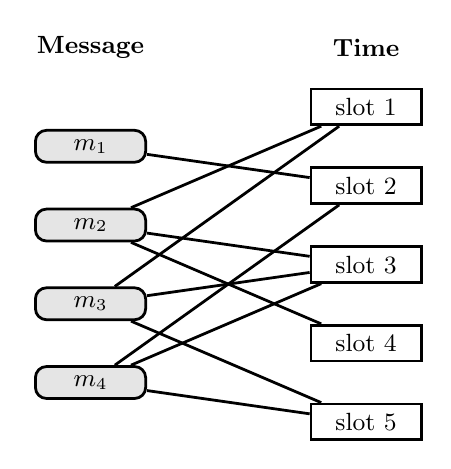
\begin{tikzpicture}
  [
  font=\small, line width=1pt, draw=black,
  bitnode/.style={circle, inner sep = 0pt, minimum size = 6mm, draw=black},
  checknode/.style={rectangle, minimum height=4mm, minimum width=14mm, draw=black},
  packet/.style={rectangle, minimum height=4mm, minimum width=14mm, draw=black, fill=gray!20, rounded corners}
  ]

\foreach \m in {1,2,3,4} {
  \node[packet] (v\m) at (0,0.5-\m) {$m_{\m}$};
}
  
\foreach \s in {1,2,3,4,5} {
  \node[checknode] (c\s) at (3.5,1-\s) {slot~\s};
}

\node (message) at (0,0.75) {\textbf{Message}};
\node (time) at (3.5,0.75) {\textbf{Time}};

\draw (v1) -- (c2);
\draw (v2) -- (c1);
\draw (v2) -- (c3);
\draw (v2) -- (c4);
\draw (v3) -- (c1);
\draw (v3) -- (c3);
\draw (v3) -- (c5);
\draw (v4) -- (c2);
\draw (v4) -- (c3);
\draw (v4) -- (c5);
\end{tikzpicture}

